\section{Intelligence Artificielle}

\subsection{Stratégies}
    \subsubsection{Intelligence aléatoire}
        Lorsque le personnage est dans une salle de combat, il joue aléatoirement des cartes jusqu'à une éventuelle fin de combat. Il peut aussi choisir de finir son tour. Lorsqu'il est dans la salle de repos, il choisira aléatoirement entre se soigner ou améliorer ses statistiques. Lorsqu'il est dans une salle d'entrainement ou si le joueur à remporté un combat, le personnage choisira aléatoirement une carte parmis les trois proposées pour rajouter à son deck, ou choisira de passer à la salle suivante directement. Si il est à l'exterieur d'une salle, et donc sur la carte, la seule option disponible est de rentrer dans la salle suivante.
    
    \subsubsection{Intelligence basée sur des heuristiques}
        Nous proposons un ensemble d'heuristiques pour chaque salle:
        \begin{itemize}
            \item \textbf{Salle de repos:} Si le joueur a moins de 50\% de sa vie, il choisira de se soigner. Dans le cas contraire il méditera afin de gagner de l'attaque et du block définitifs.
            \item \textbf{Salle d'entrainement:} Dans cette salle, le joueur peut choisir entre 3 cartes. Il y a des cartes considérées comme offensives (les cartes qui attaquent, et/ou débuff les ennemis) et d'autres commes défensives (soin/block ainsi que les buffs). Afin de choisir une carte à rajouter au deck, le joueur va essayer d'avoir le même nombre de cartes offensives que de cartes défensives. Afin que son deck s'améliore, on oblige toujours l'IA a prendre une carte, même quand son deck est plein, et on retire une carte possédant le score le plus faible du deck. Ce score est choisi de manière arbitraire en fonction de toutes les caractéristiques de la carte, de telle sorte que les cartes du deck de départ soient les premières à être supprimées.
            \item \textbf{Salle d'ennemis:} Durant le combat, le joueur effectue un certain nombre d'étapes:
            \begin{itemize}
                \item \textbf{\'Etape 1:} Si le joueur est attaqué et qu'il n'a pas de buff "evade" sur lui, et si le joueur a dans les mains une carde donnant le buff "evade", il va la jouer.\footnote{La carte fournissant le buff "evade" étant unique et la plus coûteuse, elle ne serait pas jouée sinon, bien qu'elle donne un avantage certain.}
                \item \textbf{\'Etape 2:} S'il n'a pas le buff evade appliqué sur lui, il va ensuite essayer de blocker les dégats que vont lui infliger les ennemis, jusqu'à ce qu'il n'ait plus d'énergie suffisante, de carte de block/soin, ou que l'intégralité des dégats des ennemis soient bloqués.
                \item \textbf{\'Etape 3:} S'il en a la capacité, le joueur va ensuite d'attaquer les ennemis. Il va sélectionner le plus faible, et lui faire des dégats s'il peut faire baisser sa vie (et non juste son block). Dans le cas contraire il n'attaquera pas.
                \item \textbf{\'Etape 4:} S'il lui reste de l'énergie après toutes ces étapes, il va jouer le reste de ses cartes aléatoirement.
                \item \textbf{Fin du combat:} En fin de combat, le joueur pourra choisir une carte à ajouter à son deck, il la choisira de la m\^eme manière qu'il choisit des cartes dans la salle d'entrainement.
            \end{itemize}
            L'élément du joueur et des ennemi est ici considéré. L'eau infligera plus de dégat à l'air, lui sur le feu, lui sur la terre et enfin cette dernière sur l'eau. De manière générale lors d'un combat, le joueur joue prioritairement les cartes dont les éléments lui sont défavorables, afin d'essayer de terminer le tour en étant d'un autre élément et ainsi ne pas fausser le calcul du block. Si à l'étape 4, il ne lui reste que des cartes à jouer d'un élément défavorable, il n'en jouera aucune. On n'empêche cependant pas le joueur de jouer des cartes aux étapes 1, 2, 3.
        \end{itemize}
    \clearpage
    
\subsection{Conception logiciel}
    Le diagramme des classes pour l’intelligence artificielle est présenté en \autoref{uml:ai}.
    
    \underline{\textbf{AI\_Random}}
    \par Classe implantant l'intelligence aléatoire.
    
    \underline{\textbf{AI\_Heuristic}}
    
    \clearpage
    
    \begin{figure}[hp]
    \includegraphics[width=0.6\paperheight]{images/ai.png}
    \caption{\label{uml:ai}Diagramme des classes d'intelligence artificielle.} 
    \end{figure}
    
    \clearpage
    %\begin{landscape}
    %\begin{figure}[p]
    %\includegraphics[width=0.9\paperheight]{ai.pdf}
    %\caption{\label{uml:ai}Diagramme des classes d'intelligence artificielle.} 
    %\end{figure}
    %\end{landscape}

